%----------------------------------------------------------------------------------------
%	PACKAGES AND OTHER DOCUMENT CONFIGURATIONS
%----------------------------------------------------------------------------------------
\documentclass[11pt,a4paper]{article}

\usepackage[utf8]{inputenc} % to encode the document so that we can use more caracters (like Latin ones)
\usepackage[T1]{fontenc} % to encode the document so that we can use more caracters (like Latin ones)
\usepackage[english]{babel} % to write in English

\usepackage{geometry} % the paper's format and marges
\geometry{hmargin=2.3cm,vmargin=1.7cm}

\usepackage{titling} % to put the title where I want

% maths packages
\usepackage{mathtools}
\usepackage{amsmath,amsbsy}
\usepackage{bm}
\usepackage{bigints}
\usepackage{stmaryrd}
\usepackage{amsfonts}

% graphs packages
\usepackage{graphicx}
\usepackage{float}
\usepackage{caption}
\usepackage{subcaption}
\usepackage{wrapfig,epsfig}

\usepackage{color}

\newtheorem{theorem}{Theorem}[section]
\newtheorem{lemma}[theorem]{Lemma}
\newtheorem{proposition}[theorem]{Proposition}
\newtheorem{corollary}[theorem]{Corollary}

\newenvironment{proof}[1][Proof]{\begin{trivlist}
		\item[\hskip \labelsep {\bfseries #1}]}{\end{trivlist}}
\newenvironment{definition}[1][Definition]{\begin{trivlist}
		\item[\hskip \labelsep {\bfseries #1}]}{\end{trivlist}}
\newenvironment{example}[1][Example]{\begin{trivlist}
		\item[\hskip \labelsep {\bfseries #1}]}{\end{trivlist}}
\newenvironment{remark}[1][Remark]{\begin{trivlist}
		\item[\hskip \labelsep {\bfseries #1}]}{\end{trivlist}}

\newcommand{\qed}{\nobreak \ifvmode \relax \else
	\ifdim\lastskip<1.5em \hskip-\lastskip
	\hskip1.5em plus0em minus0.5em \fi \nobreak
	\vrule height0.75em width0.5em depth0.25em\fi}

\usepackage{vmargin}
\setmarginsrb{0.5cm}{0.5cm}{1cm}{1cm}{0cm}{0cm}{0cm}{0cm}

\usepackage[final]{pdfpages}

\usepackage{algorithm}
\usepackage{algorithmic}
%----------------------------------------------------------------------------------------
%DOCUMENT
%----------------------------------------------------------------------------------------

\begin{document}

\begin{center}
	\textbf{Contrainte geometrique de cercle par section - 22/01/2018}
\end{center}

	
\section*{Formulation de la contrainte de cercle}

\subsection*{Objectif}
On cherche à ce que chaque couche de construction de la pièce soit un cercle (le cercle de même aire  et de même barycentre que ceux de la pièce pour la section considérée), c'est-à-dire que $\forall z\in [0,H]$, il faut minimiser
\begin{equation}
\label{eq:defC1}
\int_{\partial\Omega\cap (z=h)}d_{\mathcal{C}(\Omega\cap (z=h))}(s)^2ds
\end{equation}
 avec 
 \begin{equation}
 \label{eq:explicitdist}
d_{\mathcal{C}(\Omega\cap (z=h))}(x)=\sqrt{\Bigg(X(x)-\frac{\int_{\Omega\cap (z=h)}X(x)dx}{\int_{\Omega\cap (z=h)}dx}\Bigg)^2+\Bigg(Y(x)-\frac{\int_{\Omega\cap (z=h)}Y(x)dx}{\int_{\Omega\cap (z=h)}dx}\Bigg)^2}-\sqrt{\frac{\int_{\Omega\cap (z=h)}dx}{\pi}}
 \end{equation}
 
 
 
\subsection*{Problème d'optimisation}

On s'intéresse donc au problème suivant:

\begin{equation}
\label{eq:objF}
\min_{\Omega}J(\Omega)=\int_{\partial\Gamma_N}g(s)u(s)ds 
\end{equation}

tel que, pour $\alpha$ donné,

\begin{equation}
\label{eq:constraint}
P(\Omega)=\int_{0}^{H}P_h(\Omega)dh=\int_{0}^{H}\Bigg[\int_{\partial\Omega\cap (z=h)}d_{\mathcal{C}(\Omega\cap (z=h))}(x)^2dx\Bigg]dh<\alpha
\end{equation}

où $u\in H^1(\Omega)$ l'unique solution du problème élastique suivant (avec $\partial\Omega=\Gamma\cup\Gamma_N\cup\Gamma_D$ et $\Gamma\cap\Gamma_N=\Gamma_N\cap\Gamma_D=\Gamma_D\cap\Gamma=0$):
\begin{equation}
\label{eq:pbEl}
\left\{
\begin{array}{lll}
-div\big(Ae(u)\big) & =0 & \textrm{in\,\,}\Omega \\
Ae(u).n & =g & \textrm{on\,\,}\Gamma_N \\
Ae(u).n& =0 & \textrm{on\,\,}\Gamma \\
u&=0&\textrm{on\,\,}\Gamma_D 
\end{array}
\right.
\end{equation}

\section*{Reformulation de la contrainte et dérivation}
On note $\delta_{h}(x)$ la gaussienne normalisée qui permet d'approximer la fonction de dirac qui vaut 1 lorsque $x.ez=h$ et 0 ailleurs. On a dans notre cas :
\begin{equation}
\label{eq:gaussienne}
\delta_{h}(x)=\frac{\exp \Big(-\big(Z(x)-h\big)^2*c_{g}\Big)}{\int_D \exp \Big(-\big(Z(x)-h\big)^2*c_{g}\Big)}
\end{equation}

On peut alors reconsidérer les différentes intégrales intervenant dans le problème et poser:

\begin{equation}
\label{eq:aire}
A(\Omega,h)=\int_{\Omega\cap(z=h)}dx=\int_{\Omega}\delta_{h}(x)dx
\end{equation}

\begin{equation}
\label{eq:Cx}
Cx(\Omega,h)=\int_{\Omega\cap(z=h)}X(x)dx=\int_{\Omega}\delta_h(x)X(x)dx
\end{equation}

\begin{equation}
\label{eq:Cy}
Cy(\Omega,h)=\int_{\Omega\cap(z=h)}Y(x)dx=\int_{\Omega}\delta_h(x)Y(x)dx
\end{equation}


\begin{equation}
\label{eq:Dx}
Dx(\Omega,h,.):\left\{\begin{array}{lll}
D & \mapsto & \mathbb{R} \\
x & \rightarrow & X(x)-\frac{Cx(\Omega,h)}{A(\Omega,h)}
\end{array}
\right.
\end{equation}

\begin{equation}
\label{eq:Dy}
Dy(\Omega,h,.):\left\{\begin{array}{lll}
D & \mapsto & \mathbb{R} \\
x & \rightarrow & Y(x)-\frac{Cy(\Omega,h)}{A(\Omega,h)}
\end{array}
\right.
\end{equation}

\begin{equation}
\label{eq:DE}
DE(\Omega,h,.):\left\{\begin{array}{lll}
D & \mapsto & \mathbb{R} \\
x & \rightarrow & Dx(\Omega,h,x)^2+Dy(\Omega,h,x)^2
\end{array}
\right.
\end{equation}

\begin{equation}
\label{eq:dist2}
dist(\Omega,h,.):\left\{\begin{array}{lll}
D & \mapsto & \mathbb{R} \\
x & \rightarrow & d_{\mathcal{C}(\Omega\cap (z=h))}(x)=\sqrt{DE(\Omega,h,x)}-\sqrt{\frac{A(\Omega,h)}{\pi}}
\end{array}
\right.
\end{equation}

Et la contrainte peut être reformulée sous la forme :

\begin{equation}
\label{eq:constraint2}
P(\Omega)=\int_{0}^{H}\int_{\partial\Omega}\delta_h(x)dist(\Omega,h,x)^2dxdh
\end{equation}


\subsection*{Dérivation de la contrainte}
\begin{equation}
\begin{array}{l}
P'(\Omega)(\theta)=\bigint_{0}^{H}\Bigg[\int_{\partial\Omega}\bigg(\frac{\partial\Big(\delta_h(s)dist(\Omega,h,s)^2\Big)}{\partial n}+H(s)\delta_h(s)dist(\Omega,h,s)^2\bigg)\theta(s)n(s)ds \\
\qquad \qquad \qquad \qquad \qquad \qquad \qquad \qquad \qquad +\int_{\partial\Omega}2\delta_h(s)dist(\Omega,h,s)dist'(\Omega,h,s)(\theta)ds\Bigg]dh
\end{array}
\end{equation}

\begin{equation}
\label{eq:derDist}
\begin{array}{l}
dist'(\Omega,h,x)(\theta)=\frac{DE'(\Omega,h,x)(\theta)}{2\sqrt{DE(\Omega,h,x)}}-\frac{A'(\Omega,h)}{2\sqrt{\pi A(\Omega,h)}} \\
\\
\qquad= \frac{2Dx(\Omega,h,x)Dx'(\Omega,h,x)(\theta)+2Dy(\Omega,h,x)Dy'\Omega,h,x)(\theta)}{2\sqrt{DE(\Omega,h,x)}}-\frac{A'(\Omega,h)}{2\sqrt{\pi A(\Omega,h)}}\\
\\
\qquad = \frac{-Dx(\Omega,h,x)}{A(\Omega,h)\sqrt{DE(\Omega,h,x)}}\Big(Cx'(\Omega,h)(\theta)-\frac{Cx(\Omega,h)}{A(\Omega,h)}A'(\Omega,h)(\theta)\Big)+\frac{-Dy(\Omega,h,x)}{A(\Omega,h)\sqrt{DE(\Omega,h,x)}}\Big(Cy'(\Omega,h)(\theta)-\frac{Cy(\Omega,h)}{A(\Omega,h)}A'(\Omega,h)(\theta)\Big)\\
\\
\qquad \qquad \qquad \qquad -\frac{A'(\Omega,h)}{2\sqrt{\pi A(\Omega,h)}}  \\
\\
\qquad =
\frac{-Dx(\Omega,h,x)}{A(\Omega,h)\sqrt{DE(\Omega,h,x)}}\int_{\partial\Omega}\delta_h(s')\Big(X(s')-\frac{Cx(\Omega,h)}{A(\Omega,h)}\Big)\theta(s')n(s')ds'\\
\\
\qquad \qquad  +\frac{-Dy(\Omega,h,x)}{A(\Omega,h)\sqrt{DE(\Omega,h,x)}}\int_{\partial\Omega}\delta_h(s')\Big(Y(s')-\frac{Cy(\Omega,h)}{A(\Omega,h)}\Big)\theta(s')n(s')ds'-\frac{A'(\Omega,h)}{2\sqrt{\pi A(\Omega,h)}}\\
\\
\qquad =\bigint_{\partial\Omega}\frac{-Dx(\Omega,h,x)\delta_h(s')Dx(\Omega,h,s')}{A(\Omega,h)\sqrt{DE(\Omega,h,x)}}\theta(s')n(s')ds'+\bigint_{\partial\Omega}\frac{-Dy(\Omega,h,x)\delta_h(s')Dy(\Omega,h,s')}{A(\Omega,h)\sqrt{DE(\Omega,h,x)}}\theta(s')n(s')ds'-\int_{\partial\Omega}\frac{\delta_h(s')}{2\sqrt{\pi A(\Omega,h)}}\theta(s')n(s')ds'
\end{array} 
\end{equation}

On a alors, en permuttant les intégrales,

\begin{equation}
\begin{array}{l}
\int_{\partial\Omega}2\delta_h(s)dist(\Omega,h,s)dist'(\Omega,h,s)(\theta)ds=\bigint_{\partial\Omega}\int_{\partial\Omega}\frac{-2\delta_h(s)dist(\Omega,h,s)Dx(\Omega,h,s)\delta_h(s')Dx(\Omega,h,s')}{A(\Omega,h)\sqrt{DE(\Omega,h,s)}}\theta(s')n(s')dsds'\\
\\
\qquad \quad+\bigint_{\partial\Omega}\int_{\partial\Omega}\frac{-2\delta_h(s)dist(\Omega,h,s)Dy(\Omega,h,s)\delta_h(s')Dy(\Omega,h,s')}{A(\Omega,h)\sqrt{DE(\Omega,h,s)}}\theta(s')n(s')dsds'-\bigint_{\partial\Omega}\int_{\partial\Omega}\frac{2\delta_h(s)dist(\Omega,h,s)\delta_h(s')}{2\sqrt{\pi A(\Omega,h)}}\theta(s')n(s')dsds'\\
\\
\\
\qquad = \bigint_{\partial\Omega}\overbrace{\int_{\partial\Omega}\frac{2\delta_h(s)dist(\Omega,h,s)Dx(\Omega,h,s)}{A(\Omega,h)\sqrt{DE(\Omega,h,s)}}ds}^{A^1(\Omega,h)}*(-1)\delta_h(s')Dx(\Omega,h,s')\theta(s')n(s')ds'\\
\\
\qquad \quad + \bigint_{\partial\Omega}\overbrace{\int_{\partial\Omega}\frac{2\delta_h(s)dist(\Omega,h,s)Dy(\Omega,h,s)}{A(\Omega,h)\sqrt{DE(\Omega,h,s)}}ds}^{A^2(\Omega,h)}*(-1)\delta_h(s')Dy(\Omega,h,s')\theta(s')n(s')ds'\\
\\
\qquad \quad + \bigint_{\partial\Omega}\overbrace{\int_{\partial\Omega}\frac{\delta_h(s)dist(\Omega,h,s)}{\sqrt{\pi A(\Omega,h)}}ds}^{A^3(\Omega,h)}*(-1)\delta_h(s')\theta(s')n(s')ds'\\
\\
\\
\qquad =\int_{\partial\Omega}\Big(-A^1(\Omega,h)*Dx(\Omega,h,s)-A^2(\Omega,h)*Dy(\Omega,h,s)-A^3(\Omega,h)\Big)\delta_h(s)\theta(s)n(s)ds
\end{array}
\end{equation}

\begin{equation}
\begin{array}{l}
P'(\Omega)(\theta)= \\
\\
\quad \bigint_0^H\bigg(\bigint_{\partial\Omega}
\theta(s)n(s)\Big(\frac{\partial\delta_h(s)}{\partial n}dist(\Omega,h,s)^2\\
\\
\quad +\delta_h(s)\Big[2*dist(\Omega,h,s)\frac{\partial dist(\Omega,h,s)}{\partial n}+dist(\Omega,h,s)^2H(s)-A^1(\Omega,h)Dx(\Omega,h,s)-A^2(\Omega,h)Dy(\Omega,h,s)-A^3(\Omega,h)\Big]\Big) ds\bigg)dh\\
\\
=\quad \bigint_0^H\bigg(\bigint_{\partial\Omega}
\theta(s)n(s)\Big(\frac{\partial\delta_h(s)}{\partial z}n_z(s)dist(\Omega,h,s)^2\\
\\
\quad +\delta_h(s)\Big[2*dist(\Omega,h,s)\frac{\partial dist(\Omega,h,s)}{\partial n}+dist(\Omega,h,s)^2H(s)-A^1(\Omega,h)Dx(\Omega,h,s)-A^2(\Omega,h)Dy(\Omega,h,s)-A^3(\Omega,h)\Big]\Big) ds\bigg)dh\\
\end{array}
\end{equation}



\section*{Résolution 2D}

\subsection*{Adaptation de la contrainte}
On s'intéresse d'abord à une unique section. On prend pour cela un domaine $\Omega\in\mathbb{R}^2$, domaine sur lequel on va appliquer la contrainte. En optimisant seulement selon cette contrainte et en oubliant la partie mécanique, on a le problème suivant :


\begin{equation}
\label{eq:objF2D}
\min_{\Omega}J(\Omega)=P(\Omega)= \int_{\partial\Omega}d_{\mathcal{C}((\Omega)}(x)^2dx
\end{equation}


avec 
\begin{equation}
\label{eq:explicitdist2D}
d_{\mathcal{C}(\Omega)}(x)=\sqrt{\Bigg(X(x)-\frac{\int_{\Omega}X(x)dx}{\int_{\Omega}dx}\Bigg)^2+\Bigg(Y(x)-\frac{\int_{\Omega}Y(x)dx}{\int_{\Omega}dx}\Bigg)^2}-\sqrt{\frac{\int_{\Omega}dx}{\pi}}
\end{equation}

On a alors la dérivée de forme suivante :

\begin{equation}
\begin{array}{l}
P'(\Omega)(\theta)=\bigint_{\partial\Omega}
\theta(s)n(s)\Big[2*dist(\Omega,s)\frac{\partial dist(\Omega,s)}{\partial n}+dist(\Omega,s)^2H(s)-A^1(\Omega)Dx(\Omega,s)-A^2(\Omega)Dy(\Omega,s)-A^3(\Omega)\Big] ds\\
\end{array}
\end{equation}

avec 
\begin{equation}
\label{eq:A1A2A32D}
A^1(\Omega)=\int_{\partial\Omega}\frac{2dist(\Omega,s)Dx(\Omega,s)}{A(\Omega)\sqrt{DE(\Omega,s)}}ds;\quad A^2(\Omega)=\int_{\partial\Omega}\frac{2dist(\Omega,s)Dy(\Omega,s)}{A(\Omega)\sqrt{DE(\Omega,s)}}ds; \quad 
A^3(\Omega)=\int_{\partial\Omega}\frac{dist(\Omega,s)}{\sqrt{\pi A(\Omega)}}ds
\end{equation}

\subsection*{Choix de code}
Afin de pouvoir utiliser la fonction freefem d'intégration le long d'un contour, il faut introduire une nouvelle fonction level set (distVraie dans le code, à distinguer de phi qui est la level set classique). Celle-ci décrit le même domaine que la level set classique phi, cependant, elle vaut 0 sur les bords du domaine de calcul $D$. Cette nouvelle fonction n'est pas utilisée uniquement pour calculer les intégrales mais c'est notre level set principale, c'est elle qu'on modifie dans le code (les résultats sont meilleurs de cette manière là). 

\vspace{0cm}

Le calcul de la fonction distVraie est expliqué dans la suite.

La fonction de densité utilisée pour connaitre l'aire est du type 
\begin{equation}
\label{eq:densite}
X=\epsilon 1_{distVraie>0}+(1-\epsilon)1_{distVraie\leq 0}
\end{equation}

\subsection*{Résultats et validation des choix de code}

\begin{itemize}
	\item Résultats pour une initialisation en ellipse, avec la levelset distVraie :
	\begin{figure}[H]
		\begin{minipage}{0.45\textwidth}
			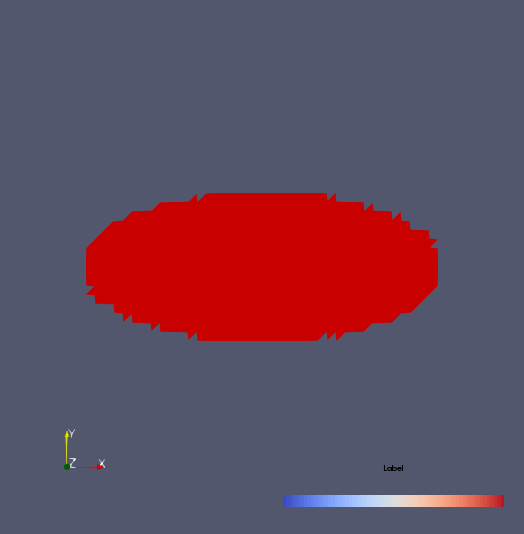
\includegraphics[width=0.9\textwidth]{SansEl2DdistVraieiniCercleINI.png}
			\caption{Initialisation}
		\end{minipage}	
		\begin{minipage}{0.45\textwidth}
			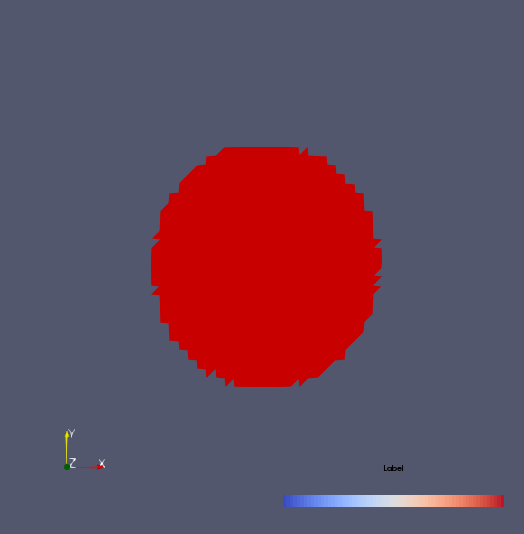
\includegraphics[width=0.9\textwidth]{SansEl2DdistVraieiniCercleResit17.png}
			\caption{Après 17 itérations}
		\end{minipage}
%		\begin{minipage}{0.3\textwidth}
%			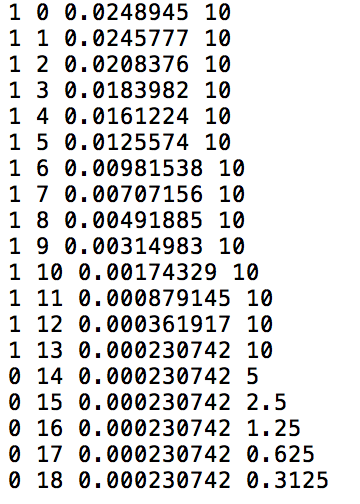
\includegraphics[width=0.9\textwidth]{val2DdistvraieINI1}
%			\caption{Valeurs}
%		\end{minipage}	
	\end{figure}
	
	\item Résultats pour une initialisation avec trous, avec la levelset distVraie :
	\begin{figure}[H]
		\label{fig:trous}
		\begin{minipage}{0.45\textwidth}
			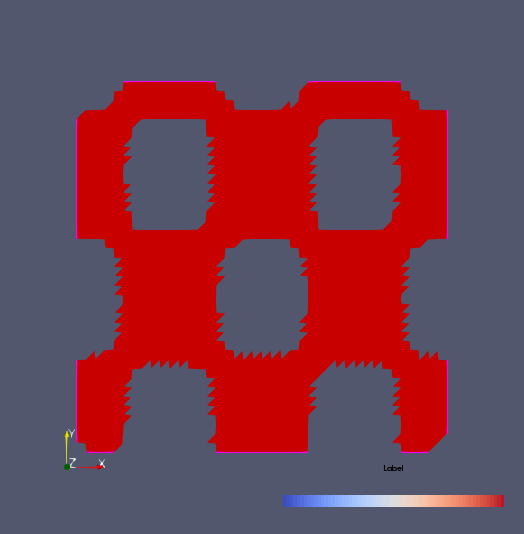
\includegraphics[width=0.9\textwidth]{SansEl2DdistVraieiniTrouINI.png}
			\caption{Initialisation}
		\end{minipage}	
		\begin{minipage}{0.45\textwidth}
			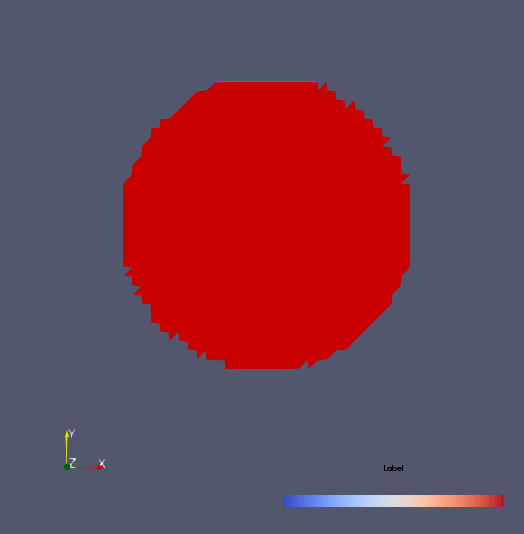
\includegraphics[width=0.9\textwidth]{SansEl2DdistVraieiniTrouResit37.png}
			\caption{Après 37 itérations}
		\end{minipage}
%		\begin{minipage}{0.3\textwidth}
%			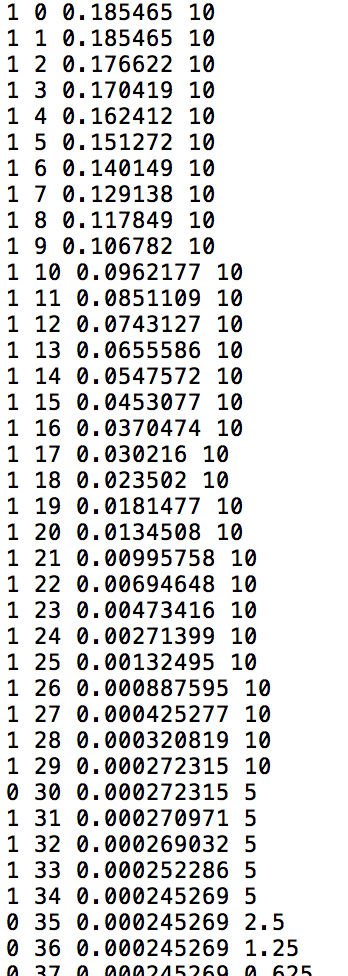
\includegraphics[width=0.9\textwidth]{val2DdistvraieINI2}
%			\caption{Valeurs}
%		\end{minipage}		
	\end{figure}	
	
	
	\item A gauche, en modifiant la fonction levelset phi, en utilisant distVraie pour les calculs d'intégrale et en utilisant phi pour les intégrales du probleme variationnel de la normale et de la vitesse. Au centre,  en modifiant la fonction levelset phi, en utilisant distVraie pour les calculs d'intégrale et pour les intégrales du probleme variationnel de la vitesse et en utilisant phi pour les intégrales du probleme variationnel de la normale. A droite, en modifiant la fonction levelset phi et en utilisant distVraie pour les calculs d'intégrale et pour les intégrales du probleme variationnel de la vitesse et de la normale. Dans tous les cas, l'initialisation est celle de la Figure \ref{fig:trous}.
	\begin{figure}[H]
		\begin{minipage}{0.3\textwidth}
			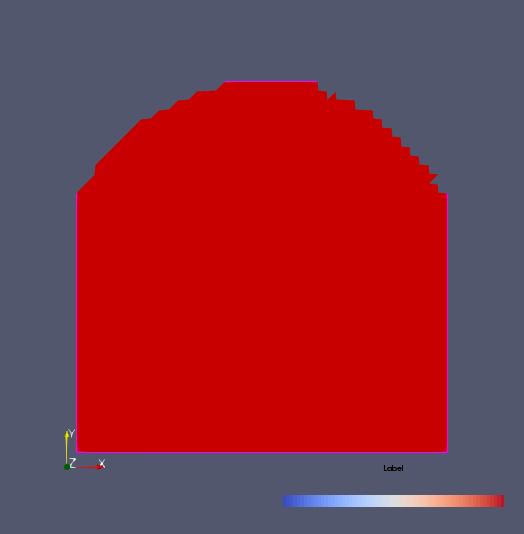
\includegraphics[width=0.9\textwidth]{SansEl2Dphinorm1vel1.png}
			\caption{Apres 56 itérations}
		\end{minipage}	
		\begin{minipage}{0.3\textwidth}
			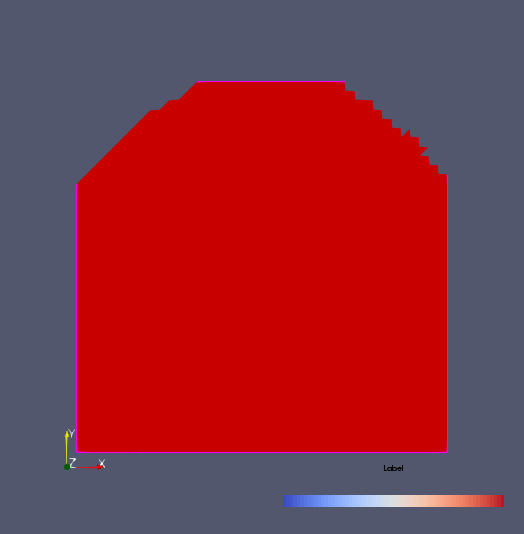
\includegraphics[width=0.9\textwidth]{SansEl2Dphinorm1vel2.png}
			\caption{Après 78 itérations}
		\end{minipage}
		\begin{minipage}{0.3\textwidth}
			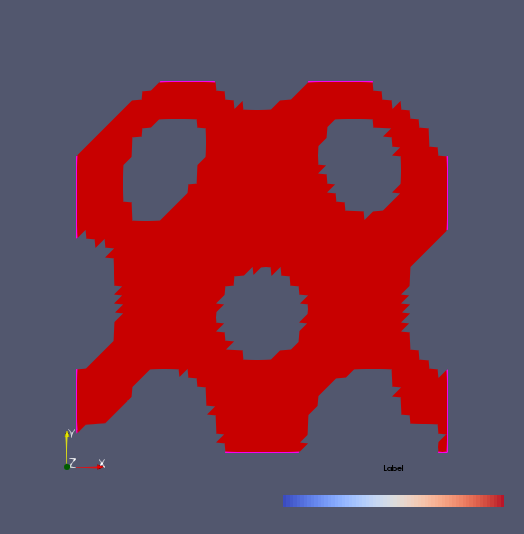
\includegraphics[width=0.9\textwidth]{SansEl2Dphinorm2vel2.png}
			\caption{Après 65 itérations}
		\end{minipage}		
	\end{figure}
	
	\item Deux types de redistanciation ont été testés (avec la fonction distance de Freefem et mshdist de Charles Dapogny). Peu de différences ont été constatés et la fonction distance a donc été retenue pour la vitesse d'exécution.
\end{itemize}



\section*{Résolution 3D, contrainte géométrique seule}

On rappelle la fonction objectif et sa dérivée de forme :

\begin{equation}
\label{eq:constraint3}
\min_{\Omega}J(\Omega)=P(\Omega)=\int_{0}^{H}\Bigg[\int_{\partial\Omega\cap (z=h)}d_{\mathcal{C}(\Omega\cap (z=h))}(x)^2dx\Bigg]dh
\end{equation}

\begin{equation}
\begin{array}{l}
P'(\Omega)(\theta)= \\
\\
\quad \bigint_0^H\bigg(\bigint_{\partial\Omega}
\theta(s)n(s)\Big(\frac{\partial\delta_h(s)}{\partial n}dist(\Omega,h,s)^2\\
\\
\quad +\delta_h(s)\Big[2*dist(\Omega,h,s)\frac{\partial dist(\Omega,h,s)}{\partial n}+dist(\Omega,h,s)^2H(s)-A^1(\Omega,h)Dx(\Omega,h,s)-A^2(\Omega,h)Dy(\Omega,h,s)-A^3(\Omega,h)\Big]\Big) ds\bigg)dh\\
\\
=\quad \bigint_0^H\bigg(\bigint_{\partial\Omega}
\theta(s)n(s)\Big(\frac{\partial\delta_h(s)}{\partial z}n_z(s)dist(\Omega,h,s)^2\\
\\
\quad +\delta_h(s)\Big[2*dist(\Omega,h,s)\frac{\partial dist(\Omega,h,s)}{\partial n}+dist(\Omega,h,s)^2H(s)-A^1(\Omega,h)Dx(\Omega,h,s)-A^2(\Omega,h)Dy(\Omega,h,s)-A^3(\Omega,h)\Big]\Big) ds\bigg)dh\\
\end{array}
\end{equation}

Afin de les calculer, on discrétise le domaine de calcul selon l'axe (Oz), en posant une décomposition régulière de pas $dh$, $(z_0=h_0,h_1,...,h_N=z_1)$. On a alors 

\begin{equation}
\label{eq:constraintdisc}
P(\Omega)=\int_{0}^{H}P_h(\Omega)dh=\sum_{i=0}^{i=N}dh\int_{\partial\Omega\cap (z=h_i)}d_{\mathcal{C}(\Omega\cap (z=h_i))}(x)^2dx
\end{equation}

\begin{equation}
\begin{array}{l}
P'(\Omega)(\theta)=\sum_{i=0}^{i=N}dh\bigg(\bigint_{\partial\Omega}
\theta(s)n(s)ds\Big(\frac{\partial\delta_{h_i}(s)}{\partial z}n_z(s)dist(\Omega,h_i,s)^2\\
\\
\quad +\delta_{h_i}(s)\Big[2*dist(\Omega,h_i,s)\frac{\partial dist(\Omega,h_i,s)}{\partial n}+dist(\Omega,h_i,s)^2H(s)-A^1(\Omega,h_i)Dx(\Omega,h_i,s)-A^2(\Omega,h_i)Dy(\Omega,h_i,s)-A^3(\Omega,h_i)\Big]\Big)\bigg)\\
\end{array}
\end{equation}

On a alors un vitesse d'advection pour chaque section (on résout le problème variationnel de régularisation de la vitesse pour chaque couche en utilisant les mêmes coefficients puis, par linéarité, on a $v=\sum_{i=0}^{i=N}dh*v_{h_i}$)


\subsection*{Choix de code}
La fonction de Dirac utilisée est celle de l'eq \ref{eq:gaussienne}. On veut cependant éviter de l'utiliser trop souvent pour ne pas perdre en précision. On construit alors un maillage particulier. Pour chaque hauteur $h_i$, on a un maillage 2D de la section, avec un label particulier.Ainsi, la section $z=h_0=z_0$ a pour label 6, la section $z=h_1=z_0+dh$ a pour label 7, la section $z=h_N=z_1$ a pour label 6+N. La figure \ref{fig:maillage} illustre cela.

\begin{figure}[H]
	\label{fig:maillage}
	\centering
	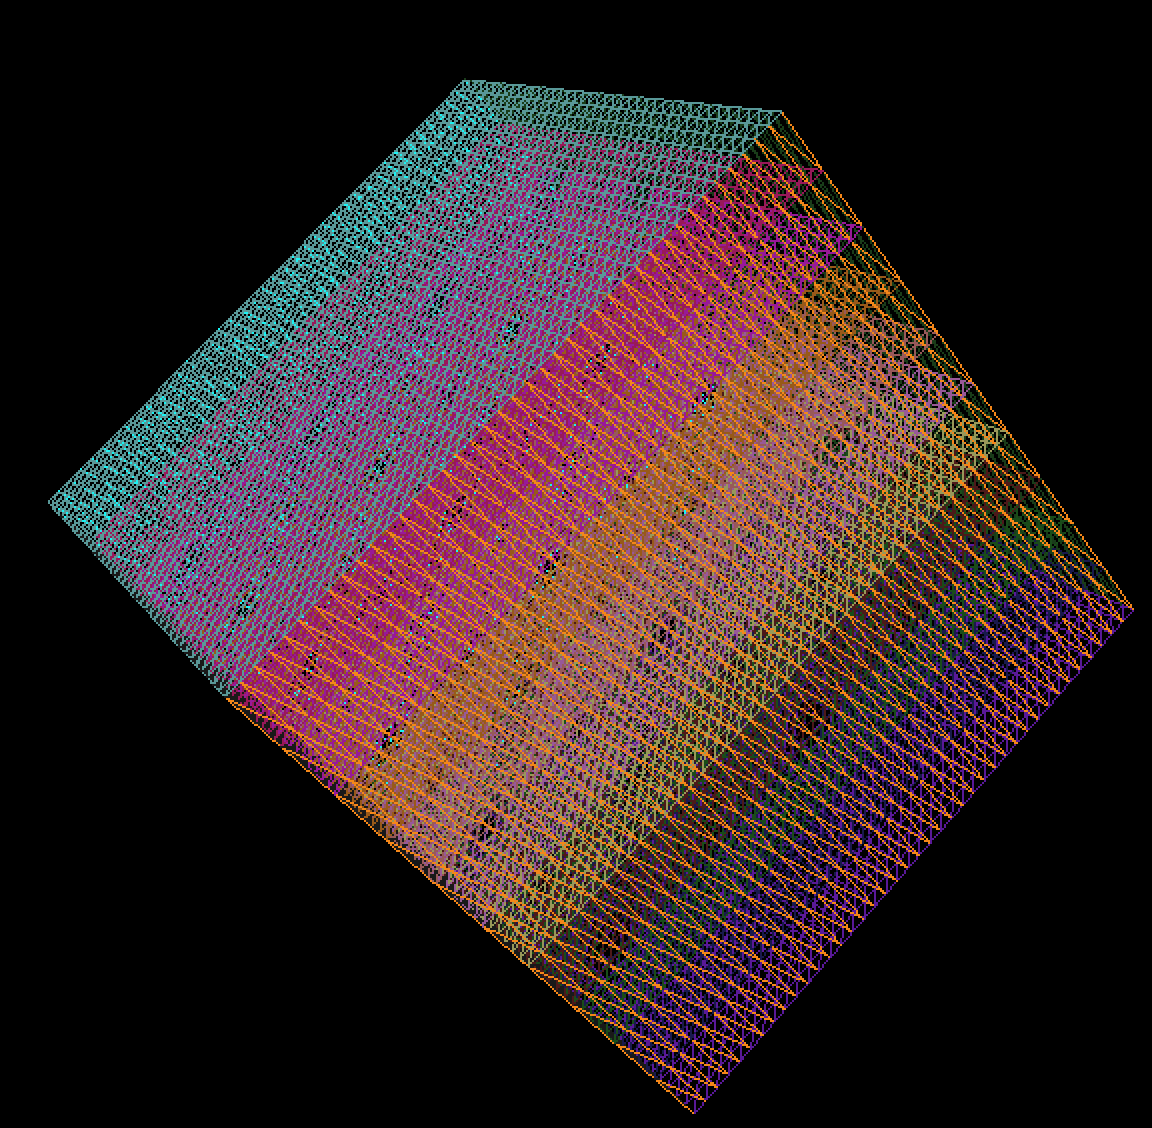
\includegraphics[width=0.4\textwidth]{mesh3D}
	\caption{}
\end{figure}

On utilise là encore une fonction différente de la level set classique comme fonction levelset. En effet, on veut à nouveau "décoller" la fonction des bords du domaine de calcul. Cependant, cette action ne doit être effectuée que sur le bords latéraux du domaine et pas sur la section inférieure ni sur la section supérieure. On itinialise donc la levelset de cette manière là et c'est cette fonction qui est advectée. Après chaque advection, on la recalcule de manière à ce qu'elle vérifie toujours cette propriété.
Afin de calculer cette fonction, on applique un probleme variationnel du type :
\begin{equation}
\begin{array}{l}
distaux=0*(phi<=0)+phi*(phi>0) \\
\\
\forall v, \int_{\Omega}distVraie*v-\int_{\Omega}\phi*v+(\textrm{on\,parois\,laterales},distVraie=distaux)
\end{array}
\end{equation}

\subsection*{Résultats}
On a ci-dessous les résultats pour une initialisation en ellipse et une initialisation de 4 trous.
\begin{figure}[H]
	\begin{minipage}{0.45\textwidth}
		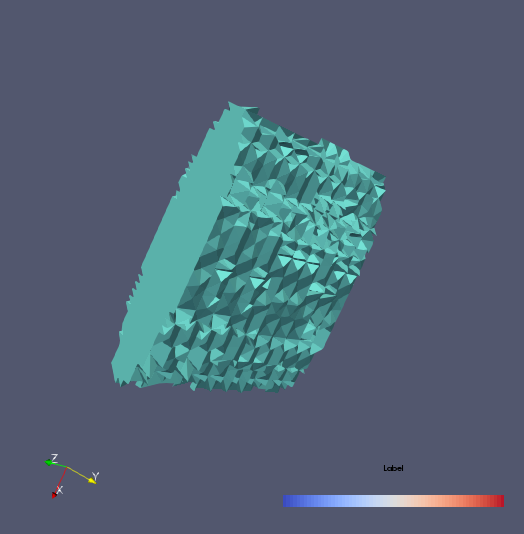
\includegraphics[width=0.9\textwidth]{SansEl3DdistVraieiniEllipseINI.png}
		\caption{Initialisation}
	\end{minipage}	
	\begin{minipage}{0.45\textwidth}
		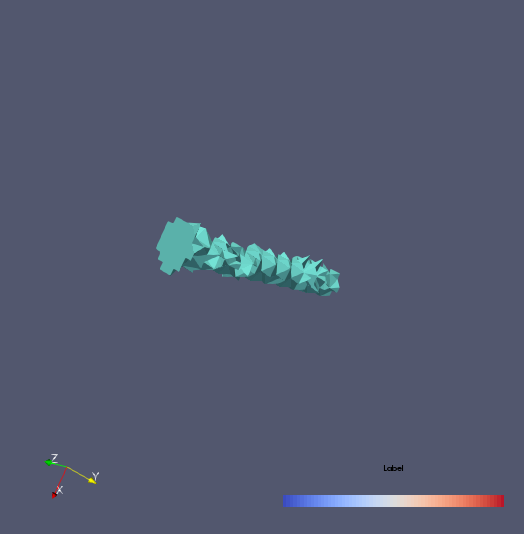
\includegraphics[width=0.9\textwidth]{SansEl3DdistVraieiniEllipseResit48.png}
		\caption{Après 48 itérations}
	\end{minipage}	
\end{figure}

\begin{figure}[H]
	\begin{minipage}{0.45\textwidth}
		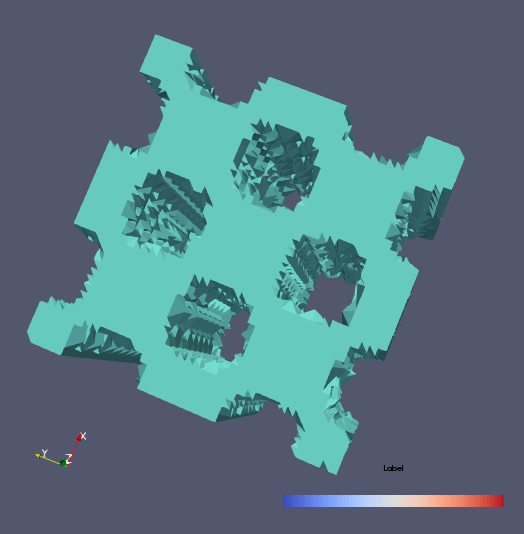
\includegraphics[width=0.9\textwidth]{SansEl3DdistVraieiniTrouINI.png}
		\caption{Initialisation}
	\end{minipage}	
	\begin{minipage}{0.45\textwidth}
		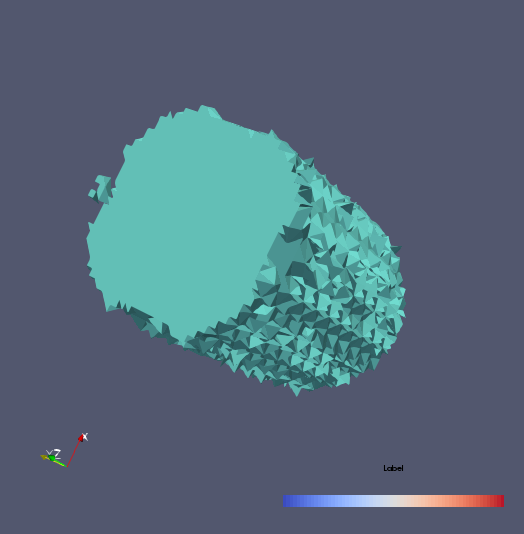
\includegraphics[width=0.9\textwidth]{SansEl3DdistVraieiniTrouResit32.png}
		\caption{Après 32 itérations}
	\end{minipage}	
\end{figure}




\section*{Resolution 3D : Minimisation de la compliance, du volume et de la contrainte}

On ajoute maintenant le problème élastique. On applique les conditions aux limites de Dirichlet sur la surface inférieure du domaine ($z=z_0$) et on applique une force selon Oy sur le centre de la surface supérieure du domaine $z=z_1$. On applique la contrainte de circularité à toutes les sections exceptée celle du haut, sur laquelle Neumann est appliquée. En revanche, la section sur laquelle Dirichlet est appliquée doit satisfaire la contrainte de circularité.

On considère le problème d'optimisation suivant :

\begin{equation}
\label{eq:objFunction}
\min_{\Omega}J(\Omega)=\int_{\partial\Gamma_N}g(s)u(s)ds 
\end{equation}

tel que,

\begin{equation}
\label{eq:volConst}
(\int_{\Omega}dx-V_{cible})^2=0
\end{equation}

et 

\begin{equation}
\label{eq:constraint3D}
P(\Omega)=\int_{0}^{H}P_h(\Omega)dh=\int_{0}^{H}\Bigg[\int_{\partial\Omega\cap (z=h)}d_{\mathcal{C}(\Omega\cap (z=h))}(x)^2dx\Bigg]dh=0
\end{equation}

où $u\in H^1(\Omega)$ l'unique solution du problème élastique suivant (avec $\partial\Omega=\Gamma\cup\Gamma_N\cup\Gamma_D$ et $\Gamma\cap\Gamma_N=\Gamma_N\cap\Gamma_D=\Gamma_D\cap\Gamma=0$):
\begin{equation}
\label{eq:pbEl2}
\left\{
\begin{array}{lll}
-div\big(Ae(u)\big) & =0 & \textrm{in\,\,}\Omega \\
Ae(u).n & =g & \textrm{on\,\,}\Gamma_N \\
Ae(u).n& =0 & \textrm{on\,\,}\Gamma \\
u&=0&\textrm{on\,\,}\Gamma_D 
\end{array}
\right.
\end{equation}


\subsection*{Multiplicateurs de Lagrange fixes pour le traitement des contraintes}
On traite les contraintes en les ajoutant à la fonction objectif, coefficientés d'un multiplicateur fixe. On a alors le problème suivant (il n'est pas nécessaire de prendre la contrainte de volume au carré car on traite ici le cas où $V_{cible}=0$) :

\begin{equation}
\label{eq:objFunction2}
\min_{\Omega}\tilde{J}(\Omega)=l_{compl}*\int_{\partial\Gamma_N}g(s)u(s)ds + l_{vol}*\Big(\int_{\Omega}dx-V_{cible})\Big)+l_{cercle}P(\Omega)
\end{equation}



\subsubsection*{Résultats}


On considère la même initialisation pour tous les cas suivant, il s'agit de l'initialisation de la figure \ref{fig:trous}.

\subsubsection*{$V_{cible}=0.\int_D dx$}

\begin{itemize}
	\item 1er cas : $l_{compl}=1;\quad l_{vol}=7; \quad l_{cercle}=10$

\begin{figure}[H]
	\begin{minipage}{0.48\textwidth}
		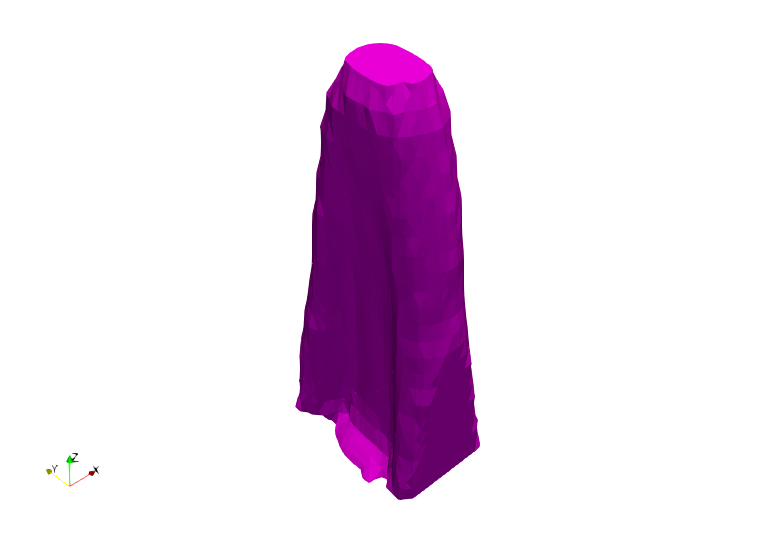
\includegraphics[width=0.9\textwidth]{it121lv7lc1lc10.png}
		\caption{Après 121 itérations}
	\end{minipage}	
	\begin{minipage}{0.48\textwidth}
		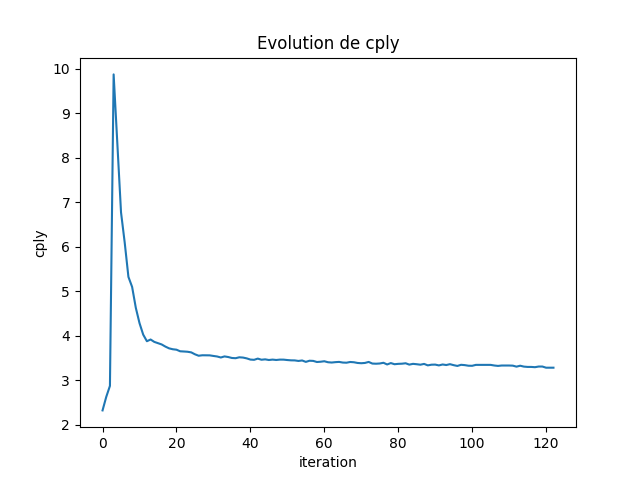
\includegraphics[width=0.9\textwidth]{lv7lc1lC10cply.png}
		\caption{Evolution de la compliance}
	\end{minipage}	
\end{figure}

\begin{figure}[H]
	\begin{minipage}{0.48\textwidth}
		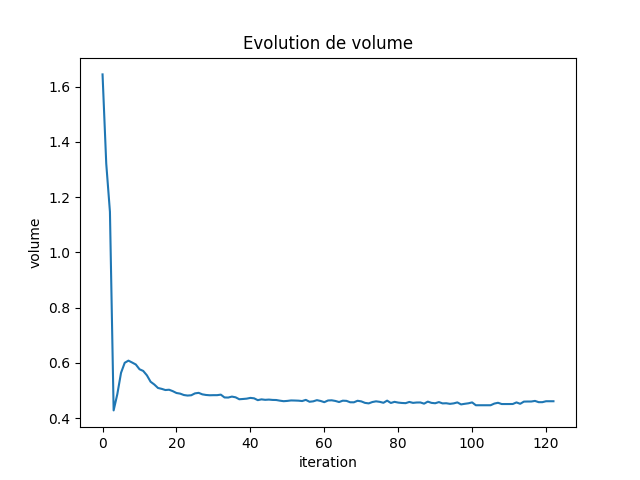
\includegraphics[width=0.9\textwidth]{lv7lc1lC10volume.png}
		\caption{Evolution du volume}
	\end{minipage}
	\begin{minipage}{0.48\textwidth}
		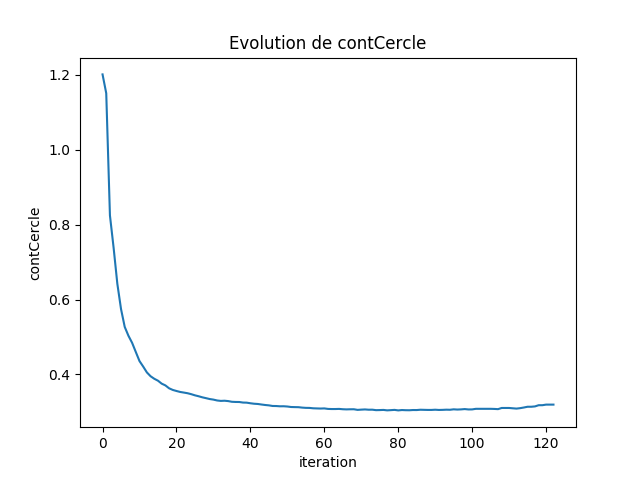
\includegraphics[width=0.9\textwidth]{lv7lc1lC10ConCercle.png}
		\caption{Evolution de la contrainte de cercle}
	\end{minipage}
\end{figure}

\item second cas : $l_{compl}=1;\quad l_{vol}=10; \quad l_{cercle}=5$

\begin{figure}[H]
	\begin{minipage}{0.48\textwidth}
		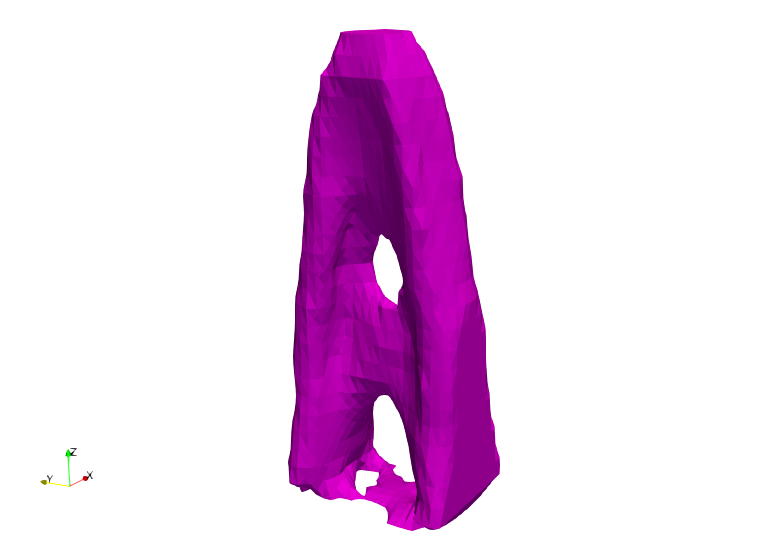
\includegraphics[width=0.9\textwidth]{it151lv10lc1lc5.png}
		\caption{Après 151 itérations}
	\end{minipage}	
	\begin{minipage}{0.48\textwidth}
		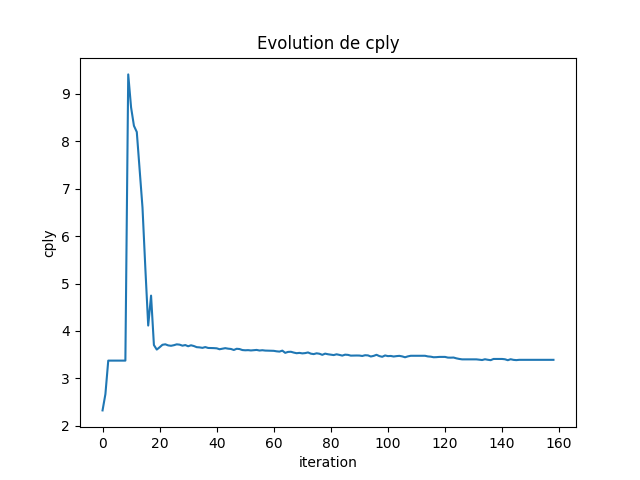
\includegraphics[width=0.9\textwidth]{lv10lc1lC5cply.png}
		\caption{Evolution de la compliance}
	\end{minipage}	
\end{figure}

\begin{figure}[H]
	\begin{minipage}{0.48\textwidth}
		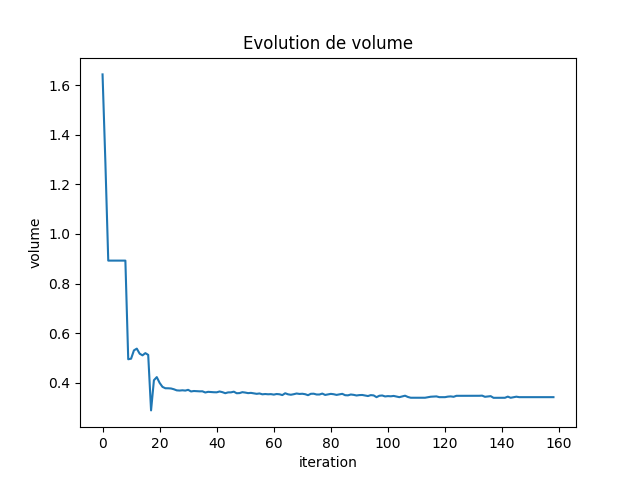
\includegraphics[width=0.9\textwidth]{lv10lc1lC5volume.png}
		\caption{Evolution du volume}
	\end{minipage}
	\begin{minipage}{0.48\textwidth}
		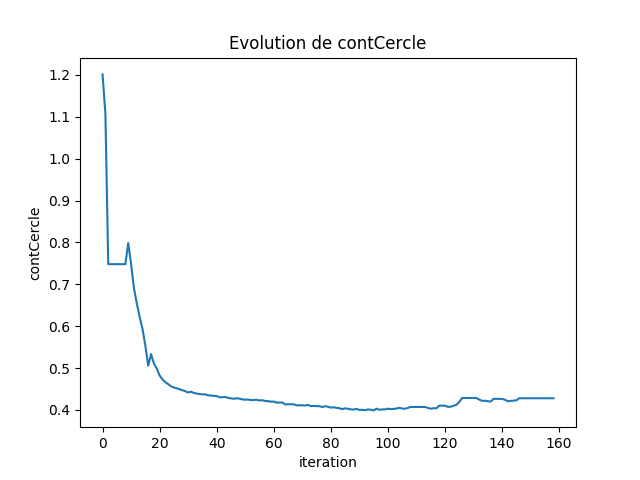
\includegraphics[width=0.9\textwidth]{lv10lc1lC5ConCercle.png}
		\caption{Evolution de la contrainte de cercle}
	\end{minipage}
\end{figure}


\end{itemize}
\subsection*{Multiplicateurs pour les contraintes non fixes}

On modifie maintenant les multiplicateurs de Lagrange en fonction du résultat de l'itération précédente. On prend ici $V_{cible}$ différent de 0 mais on n'a pas à passer la contrainte au carré car ceci est régulé naturellement par le multiplicateur de Lagrange. \textcolor{red}{Hum Hum...}

\begin{equation}
\begin{array}{l}
l_{Vol}=0.5*\frac{\int_{\partial\Omega}(-Ae(u)e(u))ds}{\int_{\partial\Omega}1ds}+\textrm{step}\frac{\textrm{Vol}-V_{cible}}{V_{cible}} \\
\\
l_{Cercle}=\left\{\begin{array}{ll}
0 & \textrm{si\,}P(\Omega)\leq 0 \\
l_{Cercle}+\textrm{step\,}P(\Omega) & \textrm{sinon}
\end{array}\right.
\end{array}
\end{equation}


On a alors le résultat suivant :

\begin{figure}[H]
	\begin{minipage}{0.48\textwidth}
		\includegraphics[width=0.9\textwidth]{toutnonfixe.png}
		\caption{Après 81 itérations}
	\end{minipage}	
	\begin{minipage}{0.48\textwidth}
		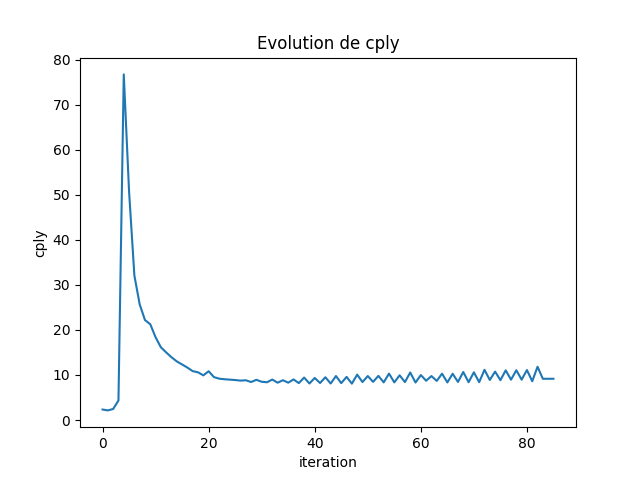
\includegraphics[width=0.9\textwidth]{toutNonFixecply.png}
		\caption{Evolution de la compliance}
	\end{minipage}	
\end{figure}

\begin{figure}[H]
	\begin{minipage}{0.48\textwidth}
		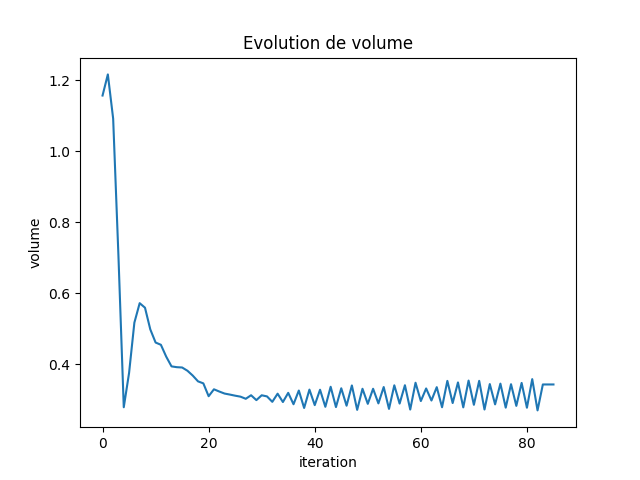
\includegraphics[width=0.9\textwidth]{toutNonFixevolume.png}
		\caption{Evolution du volume}
	\end{minipage}
	\begin{minipage}{0.48\textwidth}
		\includegraphics[width=0.9\textwidth]{toutNonFixeContCercle.png}
		\caption{Evolution de la contrainte de cercle}
	\end{minipage}
\end{figure}


%
%\subsection*{Sans permutation}
%Si on décide de ne pas permuter les intégrales, il faut alors donner une subdivision $(h_0,...h_N)$ de $[0,H]$ et on aura dans ce cas :
%\begin{equation}
%\label{eq:sansPermuter}
%P'(\Omega)(\theta)=\sum_{i=0}^{i<N} \int_{\partial\Omega} \Delta h *\delta_{h_i}(s) \Big(dist(\Omega,h_i,s)^2+A_1(\Omega,h_i)+A_2(\Omega,h_i)X(s)+A_3(\Omega,h_i)Y(s)\Big)\theta(s)n(s)ds
%\end{equation}
%
%On régularise donc la vitesse pour chaque $i$ et on somme (tout est linéaire).
%
%
%\subsection*{Si on permute}
%On a alors 
%
%\begin{equation}
%\label{eq:avecPermutation}
%P'(\Omega)(\theta)=\int_{\partial\Omega}\theta(s)n(s)\int_0^H \delta_h(s)\Big[dist(\Omega,h,s)^2+A_1(\Omega,h)+A_2(\Omega,h)X(s)+A_3(\Omega,h)Y(s)\Big]dhds
%\end{equation}
%
%On considère que $\delta_h(s)=0$ si $h\not= Z(s)$ et donc 
%
%\begin{equation}
%\label{eq:finalPermutation}
%P'(\Omega)(\theta)=\int_{\partial\Omega}\bigg(dist\big(\Omega,Z(s),s\big)^2+A_1\big(\Omega,Z(s)\big)+A_2\big(\Omega,Z(s)\big)X(s)+A_3\big(\Omega,Z(s)\big)Y(s)\bigg)\theta(s)n(s)ds
%\end{equation}
\end{document}
